\begin{figure*}[!htbp]
\centering
   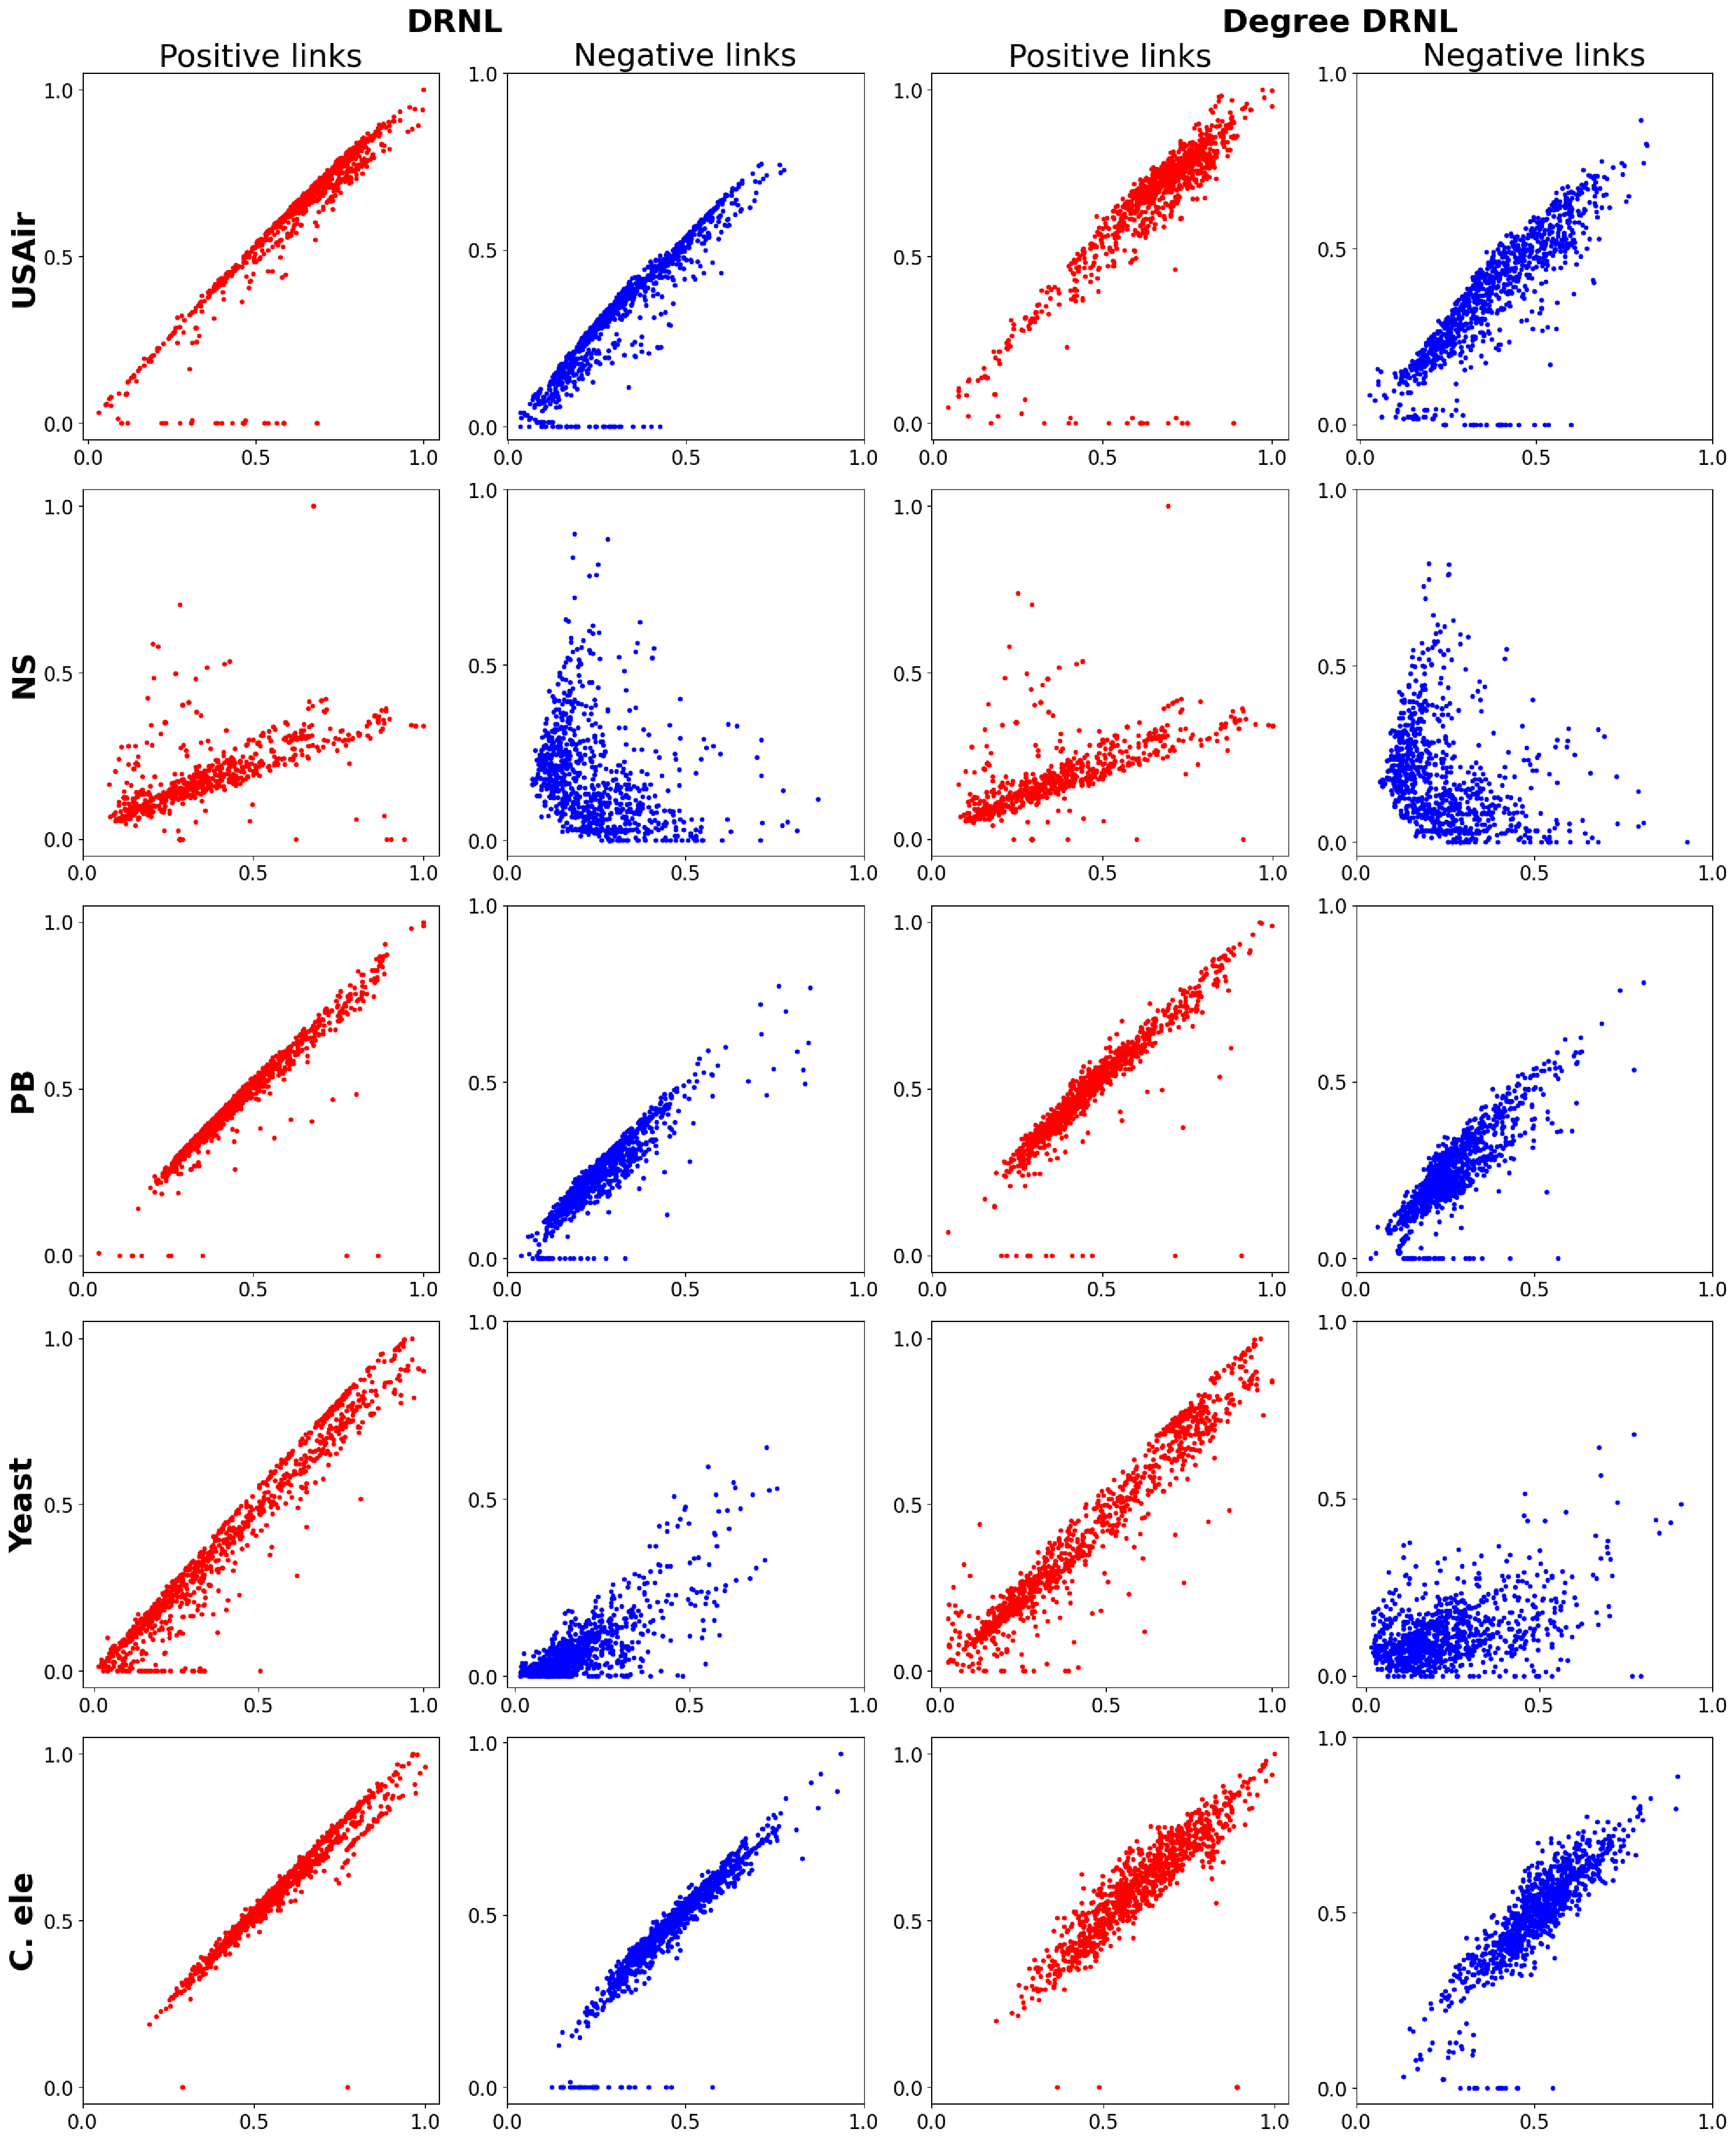
\includegraphics[width=0.9\linewidth]{figures/drnl_degdrnl_posneg1.pdf}
   \hfil
   \caption{Visualization of vectors calculated using MA-PHLP (dim0). For each dataset, the first and second columns depict the projections of persistence images (PIs) when double radius node labeling (DRNL) is applied for node labeling, and the third and fourth columns represent the values obtained when Degree DRNL is applied. 
   The first and third columns plot the values produced from positive edges (i.e., target nodes labeled $1$), and the second and fourth columns plot the values produced from negative edges (i.e., target nodes labeled $0$). }
   \label{fig:posneg1}
\end{figure*}
\begin{figure*}[!htbp]
\centering
   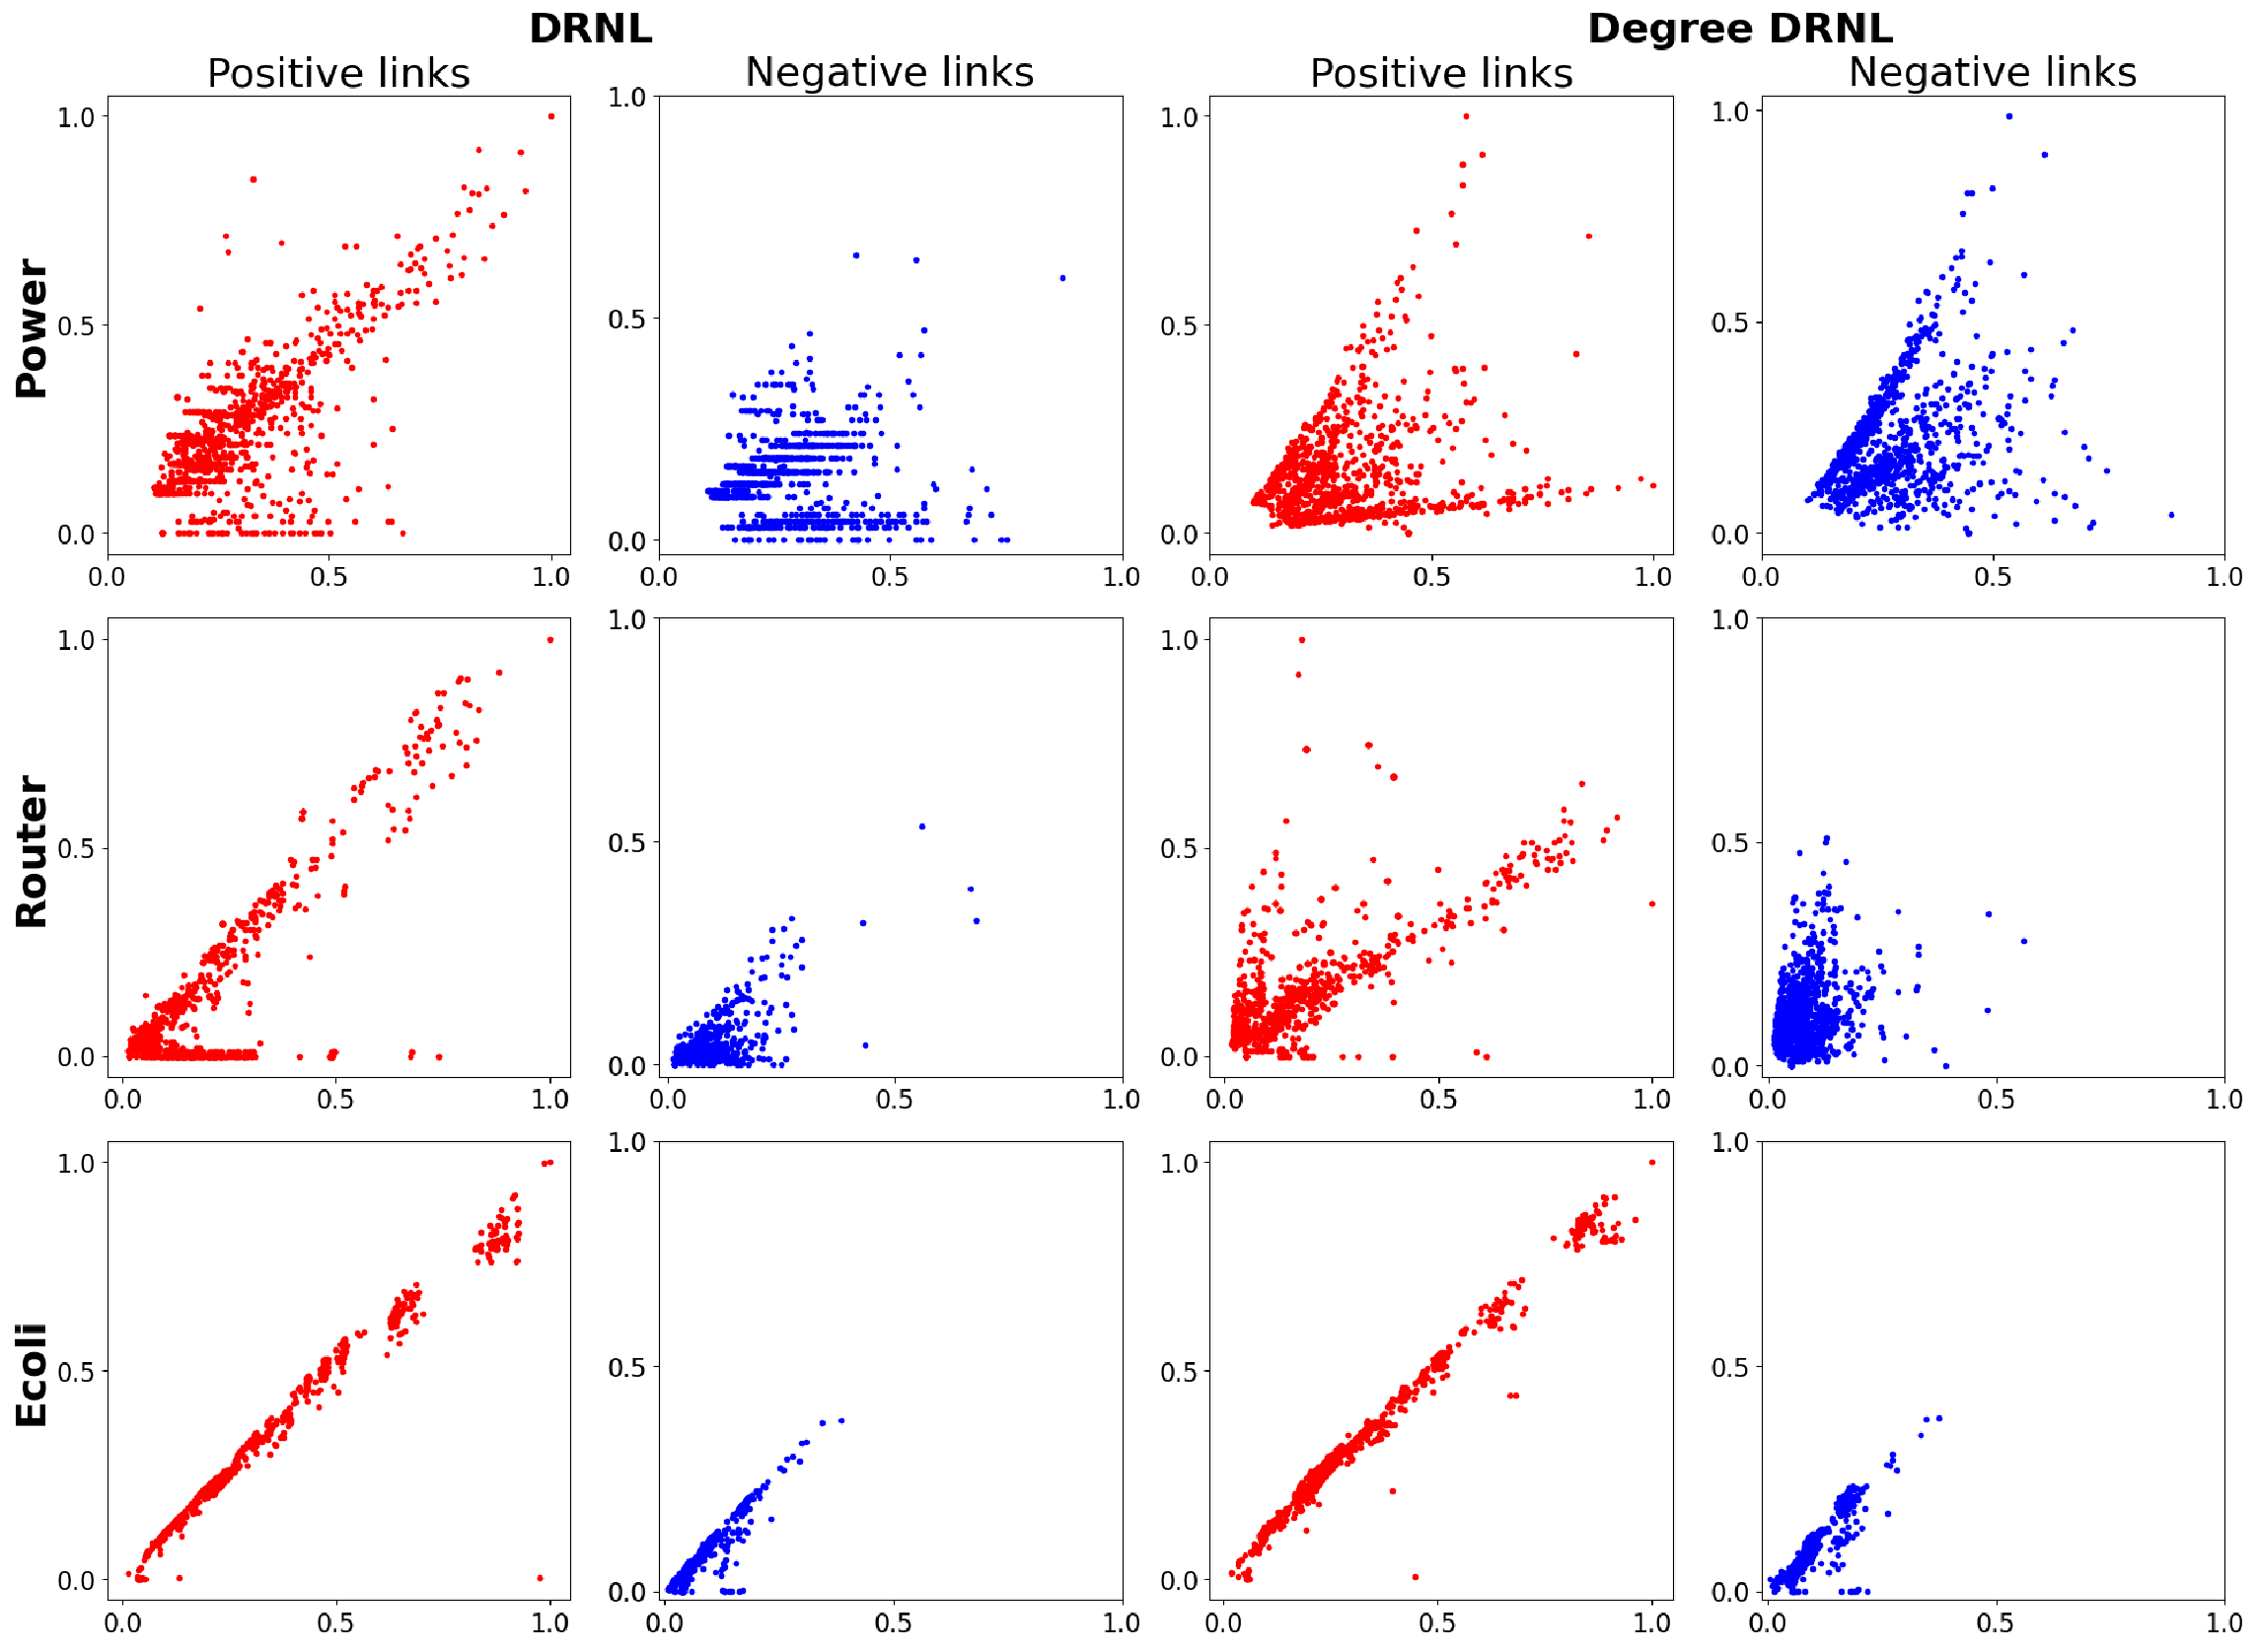
\includegraphics[width=0.9\linewidth]{figures/drnl_degdrnl_posneg2.pdf}
   \hfil
   \caption{Visualization of vectors calculated using MA-PHLP (dim0).}
   \label{fig:posneg2}
\end{figure*}


\section{Analysis}

\subsection{Analysis of the PHLP}

Figs.~\ref{fig:posneg1} and~\ref{fig:posneg2} visualize concatenated PIs to illustrate how MA-PHLP (dim0) extracts topological features for LP. 
We let $\mathcal{Z} \subseteq \mathbb{R}^{2 \times k \times r^2}$ be a set of vectors calculated by MA-PHLP, where $k$ is the number of angles, and $r$ denotes the PI resolution. 
For $(z_1, z_2) \in \mathcal{Z}$, $z_1 \in \mathbb{R}^{k \times r^2}$ is the concatenation of PIs for all angles with a target link, and $z_2 \in \mathbb{R}^{k \times r^2}$ is the concatenation for cases without a target link.
We consider a function $h:\mathbb{R}^{k \times r^2} \rightarrow \mathbb{R}$ defined as 
$h(\vec{v}_1, ..., \vec{v}_k) = \frac{1}{k}\sum_{i=1}^k \lVert \vec{v}_i \rVert_1$, where $\vec{v}_i \in \mathbb{R}^{r^2}$ are PIs, and $\lVert \cdot \rVert_1$ denotes the $L_1$-norm.
For visualization, we transform $\mathcal{Z}$ into points in $\mathbb{R}^2$ using the function $G$, defined as $G(z_1,z_2) = (h(z_1),h(z_2))$ for each $(z_1, z_2) \in \mathcal{Z}$. 

We plot distributions of points separately for positive and negative links, considering both DRNL and Degree DRNL.
The distributions of the NS and Yeast datasets between positive and negative links display significant differences, supporting the highest performance in Table~\ref{tbl:nodelabel}.
In contrast, the distributions for the C.~ele and Power datasets are the most similar when using Degree DRNL, correlating with the lowest scores in Table~\ref{tbl:nodelabel}.

\subsection{Analysis of the Power Dataset}
In most LP models, including the SOTA models SEAL and WP, the Power dataset tends to have the lowest AUC scores among the datasets. 
In Table~\ref{tbl:MA-PHLP}, the Power dataset is at the bottom in terms of scores across models (e.g., WLK, WLNM, MF, LINE, SEAL, and WP).
However, the proposed model achieves the highest AUC scores on the Power dataset among baseline models, prompting an analysis of the reasons for this performance.

In Fig.~\ref{fig:posneg2}, for DRNL, the Power dataset exhibits horizontal lines, indicating that the values $h(z_2)$ have a limited range of outcomes for vectors $z_2$ in cases without the target link; thus, the set of values $h(z_2)$ with the same value should be spread out.
This observation implies that, for numerous subgraphs the calculation of PIs yields similar outcomes despite the differences in their topological structures, posing a challenge in distinguishing between them.

To address this problem, we applied Degree DRNL, which incorporates degree information. 
The points in Fig.~\ref{fig:posneg2} are distributed without horizontal lines, leading to the highest score increase, as listed in Table~\ref{tbl:nodelabel}.

The performance of heuristic methods, such as AA, Katz, and PR, tend to be similar to random guessing on datasets with low density, particularly in the cases of the Power and Router datasets. 
Embedding methods also display low performance. 
In contrast, the GNN-based methods demonstrate improved performance using subgraphs and the network learning ability.
However, the performance for the Power dataset is significantly lower than that for the Router dataset. 

\begin{table}[h!]
\centering
\caption{Average number of nodes in subgraphs \\for the Power and Router datasets}
\label{tab:num_nodes}
\begin{tabular}{l|cc|cc}
\toprule
& \multicolumn{2}{c|}{Power} & \multicolumn{2}{c}{Router} \\
\midrule
& positive & negative & positive & negative \\
\midrule
1-hop & 8.03 & 9.12 & 5.11 & 6.72 \\
2-hop & 22.26 & 24.85 & 29.21 & 13.94 \\
3-hop & 43.11 & 49.50 & 120.35 & 55.22 \\
4-hop & 71.72 & 82.16 & 411.87 & 176.34 \\
5-hop & 99.28 & 116.75 & 740.80 & 411.35 \\
6-hop & 136.23 & 158.27 & 1272.42 & 852.13 \\
7-hop & 182.22 & 210.35 & 1835.46 & 1498.58 \\
\bottomrule
\end{tabular}
\end{table}

To bridge this gap, we analyzed subgraphs with node labeling. 
The number of nodes within the selected subgraphs between positive and negative links was significantly different on the Router dataset but not the Power dataset (Table~\ref{tab:num_nodes}). 
This difference is attributed to the presence of the hub nodes in the Router dataset, which are connected to numerous nodes. 
Thus, the subgraphs corresponding to positive links tend to have more nodes than those corresponding to negative links. 

\begin{table}[h!]
\centering
\caption{Comparison of models by Max hop settings \\on the Power and Router datasets}
\label{tab:center}
\resizebox{\linewidth}{!}{
\begin{tabular}{l|l|cccc}
\toprule
\multirow{2}{*}{\rotatebox{90}{}}& Model & MA-PHLP & MA-PHLP & WP & MA-PHLP + WP \\
\cmidrule{2-6}
& Center & target & random & - & random \\
\midrule
\multirow{7}{*}{\rotatebox{90}{Power}} & 1-hop & $78.05\pm1.20$ & $85.66\pm0.86$ & $80.24\pm0.95$ & $87.53\pm0.73$ \\
& 2-hop & $86.34\pm1.04$ & $90.52\pm0.73$ & $89.40\pm1.00$ & $91.59\pm0.77$ \\
& 3-hop & $89.65\pm0.64$ & $91.90\pm0.58$ & $\mathbf{92.11}\pm\mathbf{0.77}$ & $93.61\pm0.52$ \\
& 4-hop & $91.38\pm0.53$ & $92.67\pm0.55$ & $91.67\pm0.80$ & $94.85\pm0.55$ \\
& 5-hop & $92.27\pm0.40$ & $93.06\pm0.44$ & $91.39\pm0.78$ & $95.55\pm0.59$ \\
& 6-hop & $92.77\pm0.47$ & $93.16\pm0.49$ & $91.55\pm0.83$ & $95.85\pm0.44$ \\
& 7-hop &$\mathbf{93.06} \pm\mathbf{0.43}$  & $\mathbf{93.37} \pm\mathbf{0.41}$  & $91.50 \pm 0.89$ & $\mathbf{96.01} \pm\mathbf{0.52}$\\
\midrule
\multirow{7}{*}{\rotatebox{90}{Router}} & 1-hop & $93.12 \pm 0.45$ & $93.40 \pm 0.46$ & $94.48 \pm 0.36$ & $94.83 \pm 0.41$ \\
& 2-hop & $95.96 \pm 0.40$ & $95.70 \pm 0.45$ & $97.15 \pm 0.27$ & $97.22 \pm 0.23$ \\
& 3-hop & $96.38 \pm 0.41$ & $96.11 \pm 0.43$ & $\mathbf{97.28} \pm \mathbf{0.24}$ & $\mathbf{97.42} \pm \mathbf{0.27}$ \\
& 4-hop & $96.45 \pm 0.40$ & $96.22 \pm 0.43$ & OOM\footnotemark & OOM \\
& 5-hop & $\mathbf{96.46} \pm \mathbf{0.42}$ & $\mathbf{96.24} \pm \mathbf{0.48}$ & OOM & OOM \\
& 6-hop & $96.44 \pm 0.45$ & $96.23 \pm 0.47$ & OOM & OOM \\
& 7-hop & $96.43 \pm 0.45$ & $96.19 \pm 0.49$  & OOM & OOM \\
\bottomrule
\end{tabular}}
\end{table}
\footnotetext{OOM denotes ``out of GPU memory''.}

However, the Power dataset does not have hub nodes, and the number of nodes in the subgraph of positive links remains small. 
We randomly changed the center nodes $(a,b)$ for node labeling $f^{(a,b)}_{\text{degdrnl}}$ increasing the performance, as listed in Table~\ref{tab:center}. 
This outcome highlights that setting target nodes as the center nodes may not effectively analyze the topological structure in the case of small graphs. 
Furthermore, the performance for the Power dataset continues to increase with increasing hops (Table~\ref{tab:center}), achieving an AUC score of $95.87$, which is significantly better than that of $92.11$ for WP. 
